\chapter{Analisis}
\label{chap:analisis}

Pada bab ini akan dijelaskan analisis sistem yang sudah berjalan dan sistem yang akan dibangun. Analisis yang akan dibahas meliputi analisis \textit{use case}, analisis kelas, analisis kebutuhan fungsional dan non fungsional, dan analisis pemenuhan panduan pembangunan aplikasi \textit{android}.

\section{Analisis Sistem Kini}
%Analisis Portal Akademik Mahasiswa dan IFStudentPortal
% 

IFStudentPortal adalah situs yang diperuntukan bagi mahasiswa Teknik Informatika UNPAR\cite{herfan:15:portal}. IFStudentPortal dibuat dengan tujuan menjadi pengembangan lebih lanjut dari Portal Akademik Mahasiswa pada masanya. IFStudentPortal adalah hasil skripsi Herfan Heryandi \cite{herfan:15:portal} dan kontributor lainnya. Saat ini IFStudentPortal telah mendukung kurikulum 2018 berkat kontribusi skripsi Andrianto Sugiarto \cite{andrianto:18:portalsiam}\footnote{Mahasiswa Teknik Informatika dapat mengakses IFStudentPortal melalui URL \url{https://ifstudentportal.herokuapp.com/}}. Untuk mengakses Portal Akademik Mahasiswa, mahasiswa harus \textit{login} menggunakan akun email \textit{student}. Di halaman utama setelah login, terdapat tampilan profil mahasiswa, di sebelah kiri ada kolom menu untuk mengakses fitur-fitur IFStudentPortal seperti melihat ringkasan data akademik, melihat jadwal yang tersusun, dan melihat prasyarat mata kuliah.
\begin{figure}[H]
				\centering
				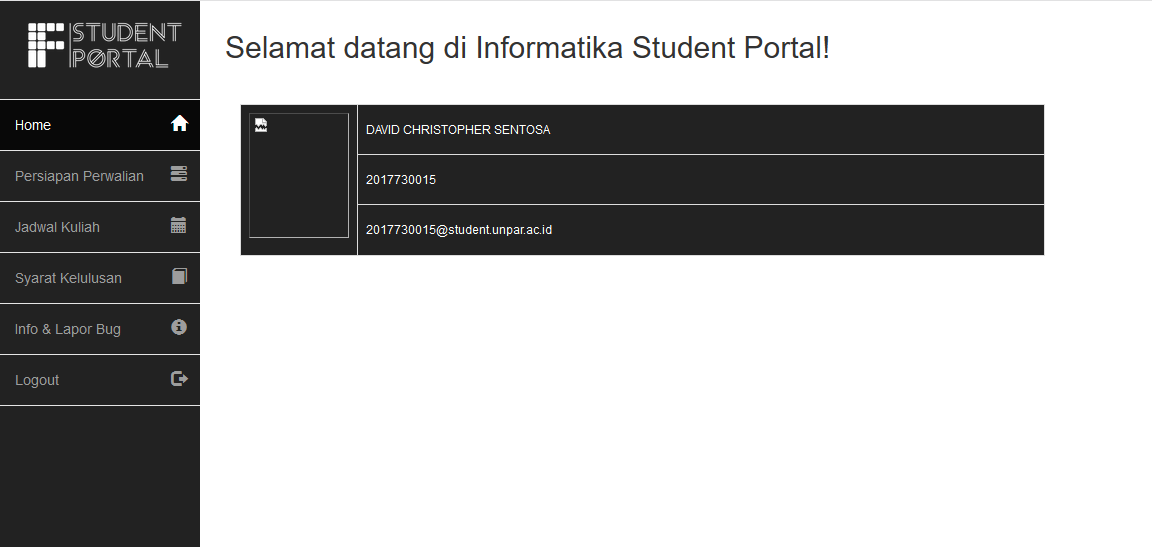
\includegraphics[scale=0.5]{Gambar/home}
				\caption{Tampilan halaman utama IFStudentPortal} 
				\label{fig:ifstudpor_home}
			\end{figure}
			
SIA Models merupakan \textit{library} Java yang merepresentasikan Sistem Informasi Akademik Teknik Informatika UNPAR \cite{siamodels}. Saat ini SIAModels mendukung kurikulum 2018. 

\subsection{Analisis Fitur IFStudentPortal}
IFStudentPortal pada awalnya dibuat untuk melengkapi informasi yang belum ada di Portal Akademik Mahasiswa pada tahun 2015. Fitur-fitur yang diimplementasikan di IFStudentPortal adalah sebagai berikut : 
\begin{enumerate}
    \item \textit{Login} : 
    Untuk dapat menggunakan situs IFStudentPortal, mahasiswa Teknik Informatika UNPAR harus \textit{login} menggunakan akun dan kata sandi yang sama dengan yang digunakan untuk \textit{login} ke Portal Akademik Mahasiswa. 
    \begin{itemize}
			\item Nama: \textit{Login}
			\item Aktor: Mahasiswa
			\item Deskripsi: \textit{Login} ke IFStudentPortal dengan membuka koneksi ke Portal Akademik Mahasiswa
			\item Kondisi awal: Mahasiswa adalah mahasiswa program studi Teknik Informatika UNPAR
			\item Kondisi akhir: Halaman utama IFStudentPortal ditampilkan 
			\item Skenario utama: \\ \\
        \begin{tabular}{|p{0.5cm} |p{6cm}| p{6cm}|}
        \hline
            No & Aksi Aktor &  Reaksi Sistem \\ \hline     
            1 & Pengguna mengakses situs IFStudentPortal &  Sistem menampilkan halaman \textit{login}\\ \hline 
            2 & Pengguna mengisi akun dan kata sandi lalu menekan tombol \textit{login} & Sistem membuka koneksi ke Portal Akademik Mahasiswa untuk melakukan pengecekan identitas \textit{login} \\ \hline 
            3 & & Jika login berhasil maka sistem akan menampilkan halaman utama IFStudentPortal\\ \hline 
        \end{tabular}
    \end{itemize}
    \begin{figure}[H]
				\centering
				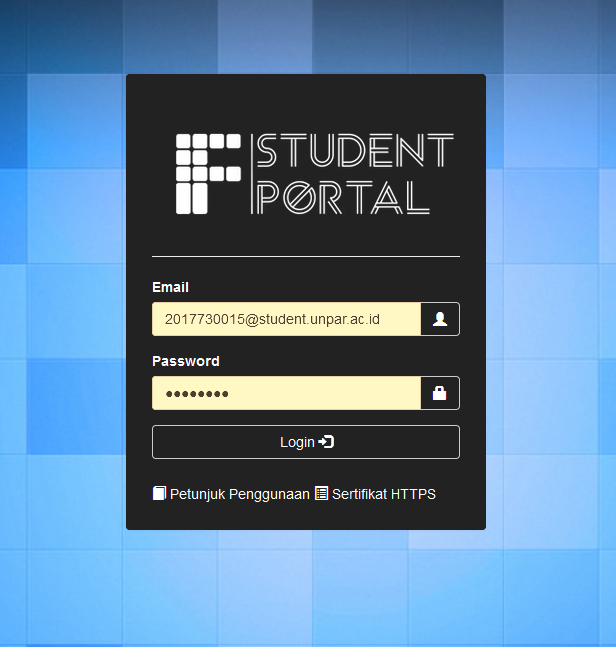
\includegraphics[scale=0.5]{Gambar/login}
				\caption{Tampilan Login} 
				\label{fig:ifstudpor_login}
			\end{figure}
    \item Prasyarat Mata Kuliah
    Mahasiswa bisa melihat mata kuliah apa saja yang dibuka di semester berjalan dan memeriksa prasyarat untuk mata kuliah tersebut. 
    \begin{itemize}
			\item Nama: Memeriksa prasyarat mata kuliah
			\item Aktor: Mahasiswa
			\item Deskripsi: Memeriksa prasyarat mata kuliah yang dibuka pada semester terkini
			\item Kondisi awal: Mahasiswa telah \textit{login}
			\item Kondisi akhir: Halaman prasyarat mata kuliah ditampilkan dan berisi mata kuliah yang dibuka pada semester terkini beserta status prasyaratnya
			\item Skenario utama: \\ \\
				\begin{tabular}{|p{0.5cm} |p{6cm}| p{6cm}|}
						\hline
							No 	& Aksi Aktor & Reaksi Sistem \\ \hline
							1 	& Mahasiswa memilih menu prasyarat mata kuliah. 	&	Sistem mendapatkan data mahasiswa kemudian menampilkan halaman prasyarat mata kuliah \\ \hline 
						\end{tabular} 
			\item Eksepsi: Mahasiswa sedang menempuh semester 1
		\end{itemize}
		\begin{figure}[H]
				\centering
				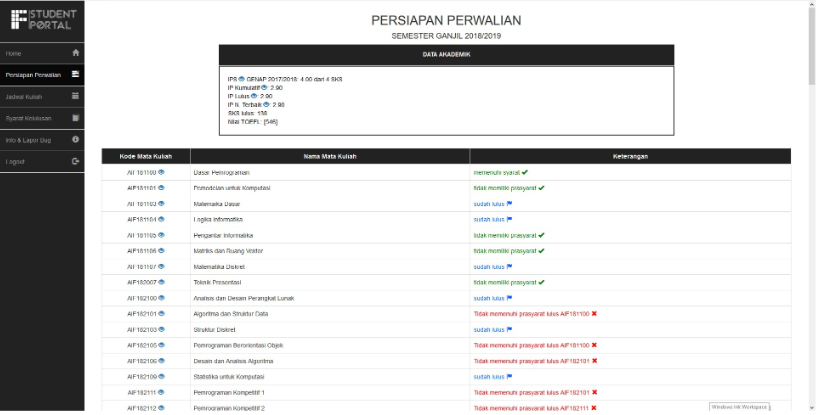
\includegraphics[scale=0.7]{Gambar/perwalian}
				\caption{Tampilan halaman daftar prasyarat mata kuliah} 
				\label{fig:ifstudpor_perwalianl}
			\end{figure}
    \item Jadwal kuliah yang tersusun
    Pada saat IFStudentPortal pertama kali dibangun, Portal Akademik Mahasiswa saat itu belum memiliki jadwal dengan tampilan grafik yang terurut berdasarkan hari dan jamnya. Fitur ini dibuat untuk mempermudah melihat susunan jadwal. 
    \begin{itemize}
			\item Nama: Melihat jadwal kuliah
			\item Aktor: Mahasiswa
			\item Deskripsi: Melihat jadwal kuliah yang sudah tersusun dan terurut berdasarkan hari dan jam
			\item Kondisi awal: Mahasiswa telah \textit{login}
			\item Kondisi akhir: Halaman jadwal ditampilkan dan berisi jadwal kuliah yang sudah tersusun dan terurut berdasarkan hari dan jam
			\item Eksepsi: Jadwal kuliah belum keluar
			\item Skenario utama: \\ \\
				\begin{tabular}{|p{0.5cm} |p{6cm}| p{6cm}|}
						\hline
							No 	& Aksi Aktor & Reaksi Sistem \\ \hline
							1 	& Mahasiswa memilih menu jadwal. 	&	Sistem menyusun dan mengurutkan jadwal mahasiswa berdasarkan hari kemudian menampilkan halaman jadwal \\ \hline 
						\end{tabular} 
		\end{itemize}
		\begin{figure}[H]
				\centering
				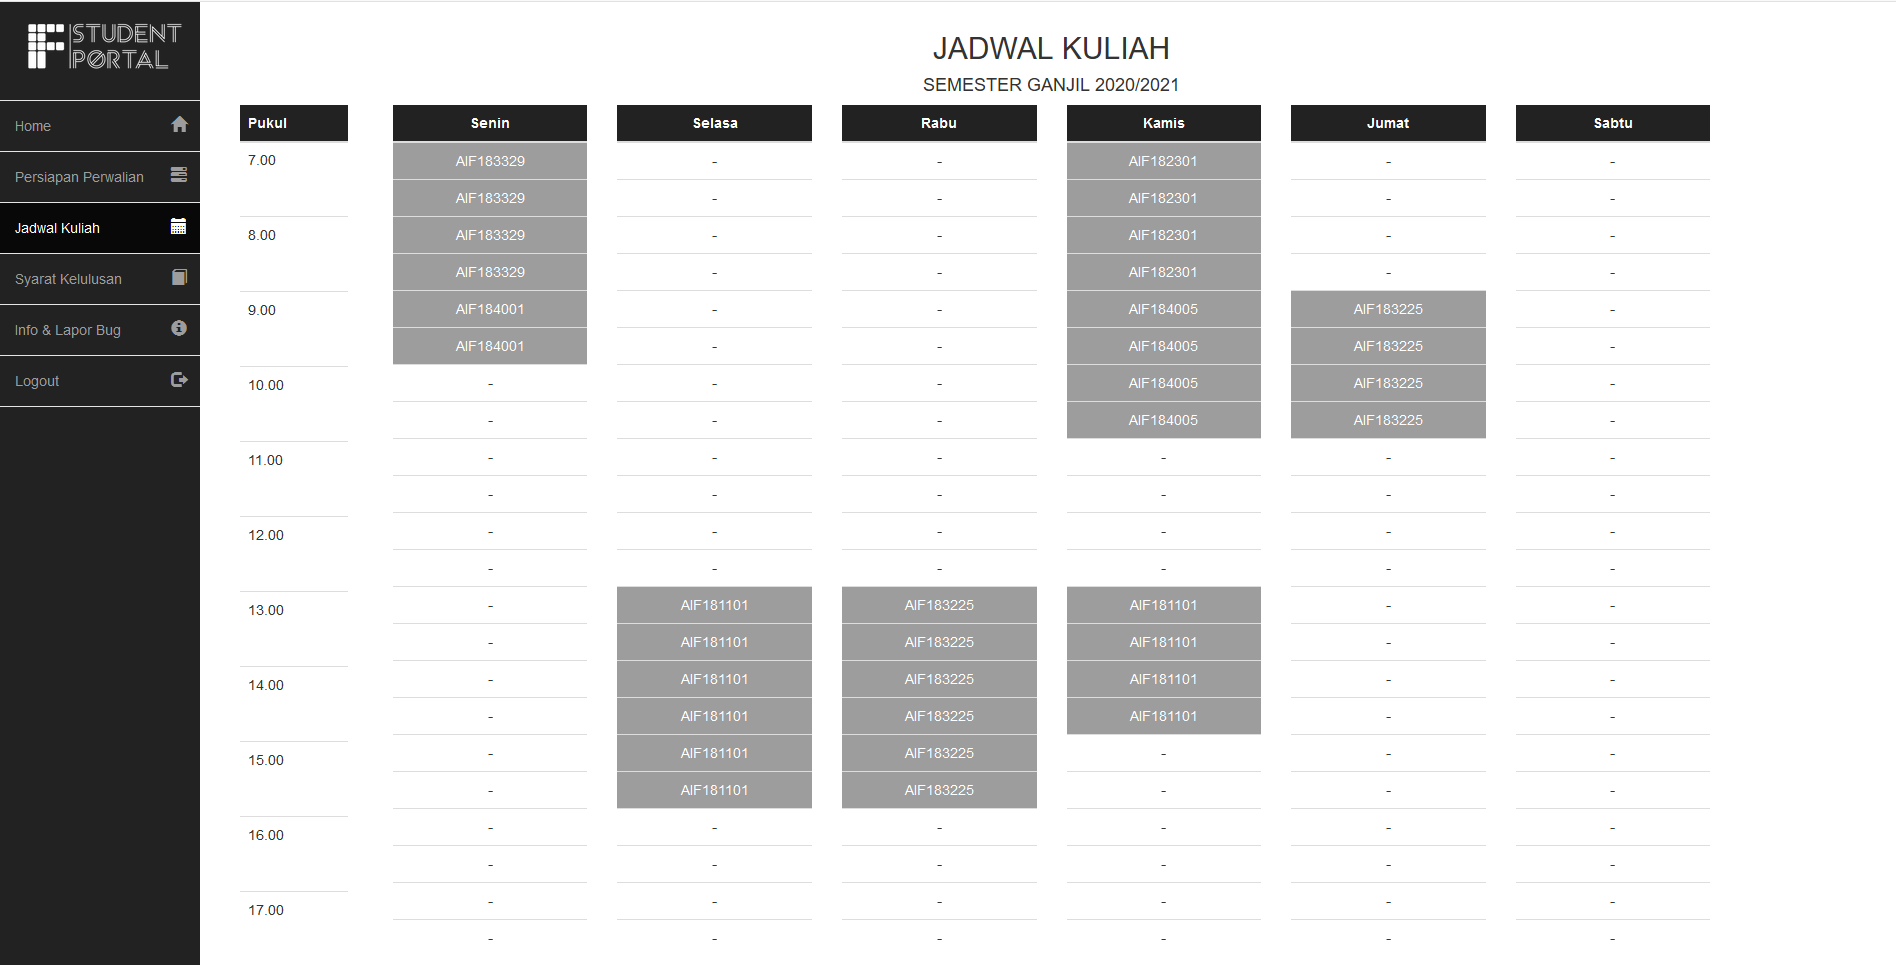
\includegraphics[scale=0.3]{Gambar/jadwal}
				\caption{Tampilan halaman jadwal kuliah yang tersusun} 
				\label{fig:ifstudpor_jadwal}
			\end{figure}
    \item Melihat ringkasan data akademik
    Pada saat IFStudentPortal pertama kali dibangun, Portal Akademik Mahasiswa saat itu belum memberikan rincian data akademik yang detil. Fitur ini dibuat untuk melengkapi informasi data akademik tersebut.
    \item \textbf{Melihat Ringkasan Data Akademik}
		\begin{itemize}
			\item Nama: Melihat ringkasan data akademik
			\item Aktor: Mahasiswa
			\item Deskripsi: melihat data mengenai mata kuliah apa saja yang sudah lulus beserta jenis mata kuliahnya(wajib atau pilihan), sisa SKS untuk mencapai kelulusan, dan mata kuliah wajib yang belum ditempuh. Mahasiswa juga dapat melihat IPS dan IPK yang lebih ter-\textit{update}
			\item Kondisi awal: Mahasiswa telah \textit{login}
			\item Kondisi akhir: Halaman yang berisi jadwal ringkasan data akademik ditampilkan
			\item Skenario utama: \\ \\
			\begin{tabular}{|p{0.5cm} |p{6cm}| p{6cm}|}
						\hline
							No 	& Aksi Aktor & Reaksi Sistem \\ \hline
							1 	& Mahasiswa memilih menu ringkasan data akademik. 	&	Sistem meringkas data akademik mahasiswa kemudian menampilkan halaman ringkasan data akademik \\ \hline 
						\end{tabular} 
		\end{itemize}
		\begin{figure}[H]
				\centering
				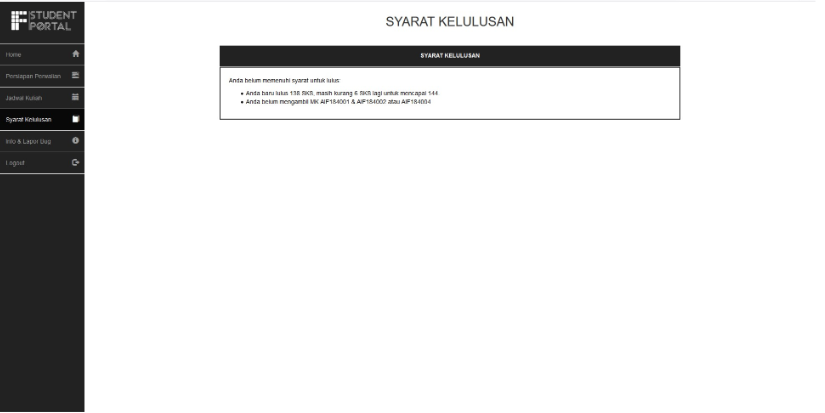
\includegraphics[scale=0.7]{Gambar/ringkasan}
				\caption{Tampilan halaman ringkasan data akademik} 
				\label{fig:ifstudpor_ringkasan}
			\end{figure}
\end{enumerate}


\section{Analisis Sistem Usulan}
IFStudentPortal akan dibangun untuk platform \textit{android}. Dokumentasi \textit{android} menyediakan panduan dalam membangun aplikasi agar aplikasi yang dibangun memiliki tampilan dan perilaku yang konsisten dengan platform \textit{android}. Panduan tersebut sudah dijelaskan di sub-bab \ref{sec:android design}. Pada sub-bab ini akan dijelaskan cara mencapai standar yang diberikan oleh panduan tersebut.

\subsection{Pemenuhan Panduan \textit{Material Design}}
Panduan aksesibilitas bertujuan memberikan arahan agar aplikasi yang dibangun mudah untuk dipelajari dan digunakan. Meningkatkan aksesibilitas akan meningkatkan kebergunaan aplikasi kepada berbagai kalangan pengguna. Berikut akan dipaparkan langkah-langkah yang dilakukan untuk meningkatkan aksesibilitas aplikasi \textit{android} IFStudentPortal :
\begin{enumerate} 
    \item (HR-01) Hierarki : 
    \begin{itemize}
        \item Warna latar belakang akan memiliki kontras yang cukup dengan warna teks.
        \item Ukuran teks akan menyesuaikan dengan ukuran layar sehingga tidak ada teks yang terlalu kecil sehingga sulit dibaca
        \item Pengisian \textit{form} akan mengalir dari atas ke bawah, dan tombol untuk \textit{submit form} tersebut akan berada di bawah form.
        \item Penyampaian informasi akan mengalir terurut dari atas ke bawah
        \item Tombol diletakan di tempat yang mudah dijangkau dengan memberikan area tekan yang besar atau meletakannya di dekat ujung layar.
    \end{itemize}
    \item (WK-01) Warna dan Kontras : 
    \begin{itemize}
        \item Warna latar belakang akan memiliki kontras yang cukup dengan warna teks.
        \item Peringatan atau pesan \textit{error} akan berwarna merah disertai dengan keterangan .
    \end{itemize}
    \item (TL-01) Tata Letak dan Tipografi : 
    \begin{itemize}
        \item Menggunakan \textit{layout} yang fleksibel dan responsif.
        \item Menggunakan format sp untuk satuan ukuran \textit{font} agar ukuran teks menyesuaikan dengan ukuran layar.
        \end{itemize}
    \item (GB-01) Gambar : 
    \begin{itemize}
        \item Melengkapi informasi yang disajikan dengan menampilkan foto profil mahasiswa.
        \end{itemize}
    % \item (NT-01) Notifikasi : 
    % \begin{itemize}
    %     \item *belum ditentukan*
    %     \end{itemize}
    \item (IA-01) Izin akses : 
    \begin{itemize}
        \item Menampilkan kotak dialog dan tombol untuk meminta izin pengguna sebelum mengakses dan mengatur kalender.
        \item Hal lain di bagian izin akses \ref{subs:izin} tidak diimplementasikan/digunakan.
        \end{itemize}
\end{enumerate}

\subsection{Pemenuhan Panduan \textit{Kualitas Aplikasi}}
Aplikasi yang berkualitas tentu saja diinginkan oleh pengguna \textit{android}. Kualitas akan mempengaruhi keberhasilan aplikasi dalam instalasi, ulasan, loyalitas, dan keterlibatan pengguna  dalam jangka panjang. Berikut akan dipaparkan langkah-langkah yang dilakukan untuk memastikan aplikasi \textit{android} IFStudentPortal memiliki kualitas yang baik :

\begin{enumerate}
    \item Desain visual dan interaksi pengguna : 
    \begin{itemize}
        \item (UX-B1) Aplikasi tidak akan menggunakan ikon yang ambigu sehingga pengguna tidak kebingungan dalam mengartikan fungsi tombol dengan ikon tersebut. 
        \item (UX-S2) Bagian ini belum memerlukan perhatian khusus %Notifikasi akan digunakan untuk memberi tahu pengguna tentang  ...  *belum ditentukan*
    \end{itemize}
    \item Fungsionalitas : 
    \begin{itemize}
        \item (FN-P1) Aplikasi akan meminta izin akses dari pengguna sebelum menggunakan kalender.
        \item (FN-L1) Bagian ini belum memerlukan perhatian khusus.
        \item (FN-A1) Aplikasi tidak menggunakan audio sebagai fitur utama.
        \item (FN-U1) Aplikasi tidak menggunakan orientasi \textit{landscape}.
        \item (FN-S1) Aplikasi akan memberhentikan layanan saat pengguna menutup aplikasi sehingga aplikasi tidak aktif saat di belakang layar.
        \item (FN-S2) Aplikasi akan mempertahankan \textit{state login} selama ada aktifitas atau sampai batas waktu yang ditentukan. 
    \end{itemize}
    \item Kompaatibilitas, Performa, dan Stabilitas : 
    \begin{itemize}
        \item (PS-S1) Aplikasi akan dibangun dengan \textit{library android} versi terbaru yang sudah stabil untuk meminimalisir kemungkinan aplikasi macet. Aplikasi akan diuji sebelum dirilis untuk memperbaiki \textit{bug} yang ditemukan.
        \item (PS-P1) Aplikasi tidak menggunakan algoritma yang kompleks dan melakukan proses yang berat sehingga tidak perlu waktu lama untuk memuat aplikasi.
        \item (PS-T1) Aplikasi dibangun dengan SDK terbaru dan diuji di perangkat terbaru dan di perangkat yang populer.
        \item (PS-M1) Aplikasi tidak memutar video dan audio sebagai fitur utama sehingga tidak memerlukan perhatian khusus.
        \item (PS-B1) Aplikasi sederhana sehingga bagian ini belum memerlukan perhatian khusus.
        \item (PS-V1) Grafik yang ditampilkan adalah gambar dengan resolusi tinggi 
    \end{itemize}
    \item Keamanan : 
    \begin{itemize}
        \item (SC-D1) Aplikasi tidak menyimpan data pengguna baik di internal maupun di log.
        \item (SC-D2) Aplikasi menggunakan data yang valid dan aman dari Portal Akademik Mahasiswa.
        \item (SC-P1) Aplikasi tidak mengekspor komponen aplikasi dengan aplikasi lain.
        \item (SC-P2) Aplikasi tidak berbagi konten dengan aplikasi lain.
        \item (SC-N1) Aplikasi membuka koneksi dengan Portal Akademik Mahasiswa yang sudah diamankan dengan SSL.
        \item (SC-N2) Bagian ini belum memerlukan perhatian khusus.
        \item (SC-U1) Aplikasi dibangun dengan \textit{dependency, library}, dan \textit{SDK} terbaru.
        \item (SC-E1) Aplikasi tidak mengeksekusi kode external secara dinamis.
        \item (SC-C1) Aplikasi tidak perlu mengenkripsi apapun.
    \end{itemize}
    \item \textit{Google Play} : 
    \begin{itemize}
        \item (GP-P1) Aplikasi tidak mengandung materi yang tidak pantas dan tidak menggunakan hak kekayaan intelektual atau merk orang lain.
        \item (GP-D1) Aplikasi akan dibangun dengan mengikuti panduan yang sudah diuraikan sebelum bagian ini.
        \item (GP-X1) Pengembang akan memperbaiki \textit{bug} yang ditemukan.
    \end{itemize}
\end{enumerate}

\subsection{Persiapan}
Sebelum dan selama proses pengembangan aplikasi \textit{android} IFStudentPortal berjalan, ada beberapa pekerjaan yang dilakukan sebagai berikut :
\begin{itemize}
    \item Perawatan situs IFStudentPortal\\
    IFStudentPortal beberapa kali mengalami gangguan sehingga tidak bisa digunakan sebagaimana mestinya, sehingga dilakukan perbaikan-perbaikan yang diperlukan. Perubahan yang dilakukan adalah sebagai berikut :
    \begin{itemize}
        \item Memperbaiki \textit{bug} alamat foto profil dari Portal Akademik Mahasiswa\footnote{Kode dapat dilihat di \url{https://github.com/ftisunpar/IFStudentPortal/commit/2534764}}.
        \item Memperbaiki \textit{bug} mengambil kode semester dari Portal Akademik Mahasiswa dengan memindahkan halaman sumber kode semester dari halaman frs ke halaman nilai\footnote{Kode dapat dilihat di \url{https://github.com/ftisunpar/IFStudentPortal/commit/4775b17}}.
        \item Merubah penggunaan SIA Models dari \textit{submodule} ke \textit{Maven}\footnote{Kode dapat dilihat di \url{https://github.com/ftisunpar/IFStudentPortal/commit/d88bba}}.
    \end{itemize}
    \item Perawatan SIA Models\\
    SIA Models versi v3.1.0 belum cocok untuk digunakan di platform \textit{android} sehingga perlu sedikit modifikasi agar bisa digunakan untuk pembangunan \textit{android} IFStudentPortal. Perubahan yang dilakukan adalah sebagai berikut :
    \begin{itemize}
        \item Merubah nilai kembalian dari \textit{method getPhotoImage} menjadi \textit{byte}\footnote{Kode dapat dilihat di \url{https:www.github.com/pascalalfadian/siamodels/commit/0df064f}.}.
    \end{itemize}
\end{itemize}

\subsection{Analisis Use Case}
Diagram \textit{use case} hanya akan memiliki 1 aktor yaitu mahasiswa Teknik Informatika UNPAR. Diagram \textit{use case} dapat dilihat di gambar \ref{}. 

Berdasarkan hasil analisis kebutuhan pada subbab \ref{kebutuhan}, dari x fitur yang akan dibuat, terdapat y buah \textit{use case} yaitu :
\begin{enumerate}
    \item \textbf{Melihat Ringkasan Data Akademik}
		\begin{itemize}
			\item Nama: Melihat ringkasan data akademik
			\item Aktor: Mahasiswa
			\item Deskripsi: melihat data mengenai mata kuliah apa saja yang sudah lulus beserta jenis mata kuliahnya(wajib atau pilihan), sisa SKS untuk mencapai kelulusan, dan mata kuliah wajib yang belum ditempuh. 
			\item Kondisi awal: Mahasiswa telah \textit{login}
			\item Kondisi akhir: Halaman ditampilkan dan berisi ringkasan data akademik
			\item Skenario utama: \\ \\
			\begin{tabular}{|p{0.5cm} |p{6cm}| p{6cm}|}
						\hline
							No 	& Aksi Aktor & Reaksi Sistem \\ \hline
							1 	& Mahasiswa memilih menu ringkasan data akademik. 	&	Sistem meringkas data kademik mahasiswa kemudian menampilkan halaman ringkasan data akademik \\ \hline 
						\end{tabular} 
			%\item Eksepsi: Mahasiswa sedang menempuh semester 1
		\end{itemize}
\end{enumerate}



\subsection{Analisis Kelas}





% Portal Akademik Mahasiswa adalah situs yang diperuntukan bagi mahasiswa UNPAR untuk mengakses informasi yang berhubungan dengan studi dan mahasiswa pemilik akun\cite{BTI:2012}. Mahasiswa dapat mengakses Portal Akademik Mahasiswa melalui URL \url{https://studentportal.unpar.ac.id/}. Untuk mengakses Portal Akademik Mahasiswa, mahasiswa harus \textit{login} menggunakan akun email \textit{student}. 

% \subsection{Analisis Kebutuhan \textit{Android} IFStudentPortal}
% \label{kebutuhan}
% Aplikasi \textit{android} IFStudentPortal akan memiliki fitur-fitur yang sudah ada di situs IFStudentPortal. Fitur-fitur tersebut akan diimplementasikan dan diintegrasikan dengan fitur-fitur \textit{android} jika memungkinkan. Untuk mengetahui fitur apa lagi yang dibutuhkan, dibuat survey untuk meminta pendapat kepada mahasiswa Teknik Informatika angkatan 2016-2020. Dari hasil survey, diperoleh fitur yang diinginkan oleh mahasiswa adalah sebagai berikut :
% \begin{itemize}
%     \item Jadwal mata kuliah yang terintegrasi dengan kalender sistem.
%     \item Notifikasi yang berisi informasi seputar perkuliahan.
%     \item Simulasi sederhana untuk masa FRS (pengecekan jadwal bentrok, jumlah sks, prasyarat).
%     \item Tempat melihat pengumuman yang bisa di urutkan dan rapi.
%     \item Tempat melihat jadwal akademik di selain jadwal kuliah mahasiswa (jam kerja Tata Usaha, jadwal tes TOEFL). 
%     \item Rincian mata kuliah (informasi presentase lulus, materi kuliah, tingkat kesulitan, dll)
%     \item Ringkasan data akademik dan syarat kelulusan
% \end{itemize}

% Fitur-fitur baru yang akan diimplementasikan akan memenuhi kriteria berikut :
% \begin{itemize}
%     \item Data yang diperlukan tersedia di Portal Akademik Mahasiswa.
%     \item Data hasil olahan tidak tersedia  di Portal Akademik Mahasiswa.
%     \item Fitur mendukung fungsi Student Portal sebagai sumber informasi akademik.
%     \item Bisa diintegrasikan dengan fitur android.
% \end{itemize}

% Hasil analisis fitur-fitur yang diinginkan berdasarkan kriteria di atas dan batas waktu pembangunan aplikasi dapat dilihat pada Tabel \ref{tab:3_hasil_fitur}.
% \begin{table}(H)
% 	\centering
% 		\caption{Tabel Hasil Analisis Kebutuhan Informatika Student Portal}
%     \begin{tabular}{|p{4.5cm}|p{2.5cm}|p{8cm}|}
% 		\hline
% 		Fitur & Dibuat/Tidak dibuat & Alasan\\
% 		\hline
% 		Simulasi FRS sederhana                      & Dibuat (mungkin)       & Data dapat diambil dari Portal Akademik Mahasiswa dan aturan prasyarat mata kuliah Program Studi Teknik Informatika sudah tersedia di SIA Models                   \\
% 		\hline
%     Tempat melihat pengumuman yang bisa di urutkan dan rapi.                               & Dibuat (mungkin)      & Data dapat diambil dari Portal Akademik Mahasiswa                       \\
% 		\hline
%     Tempat melihat jadwal akademik di selain jadwal kuliah mahasiswa (jam kerja Tata Usaha, jadwal tes TOEFL).    & Tidak Dibuat       &  Data tidak tersedia di Portal Akademik Mahasiswa \\
% 		\hline
%     Jadwal kuliah yang terintegrasi dengan kalender sistem                       & Dibuat       & Data tersedia di Portal Akademik Mahasiswa dan terintegrasi dengan fitur android                                                     \\
% 		\hline
%     Rincian mata kuliah                               & Tidak dibuat & Data tidak bisa diperoleh dari Portal Akademik Mahasiwa                                               \\
% 		\hline
%     Notifikasi yang berisi informasi seputar perkuliahan                                    & Dibuat & Data tersedia di Portal Akademik Mahasiswa dan terintegrasi dengan fitur android                                                                        \\
% 	    \hline
% 	    Ringkasan data akademik dan syarat kelulusan                                  & Dibuat & Data tersedia di Portal Akademik Mahasiswa                                                                       \\
% 	    \hline
		
% 		\end{tabular}
% 	\label{tab:3_hasil_fitur}
% \end{table}    \item \textit{Login} : 

